\documentclass[11pt,a4paper,dvipdfmx]{ujreport}

\usepackage{sotsuron}
\usepackage{here}
\usepackage{title}
\usepackage{amsmath,amssymb}
\usepackage{mathtools}
\usepackage{graphicx,color}
\usepackage[hidelinks]{hyperref} % 目次や図表番号に対してハイパーリンクを生成。hidelinks で PDF のハイパーリンクの枠を消す(参考: http://0-chromosome.hatenablog.jp/entry/2015/04/10/175912 )
\usepackage{pxjahyper} % ハイパーリンクに日本語が含まれる場合に必要
\usepackage[width=15cm]{caption}
\usepackage{longtable}
\usepackage{booktabs}
\makeatletter
\def\maxwidth{\ifdim\Gin@nat@width>\linewidth\linewidth\else\Gin@nat@width\fi}
\def\maxheight{\ifdim\Gin@nat@height>\textheight\textheight\else\Gin@nat@height\fi}
\makeatother
% Scale images if necessary, so that they will not overflow the page
% margins by default, and it is still possible to overwrite the defaults
% using explicit options in \includegraphics[width, height, ...]{}
\setkeys{Gin}{width=\maxwidth,height=\maxheight,keepaspectratio}

\usepackage[backend=biber,sorting=none]{biblatex}
\DeclarePrefChars{'-}  % https://oku.edu.mie-u.ac.jp/tex/mod/forum/discuss.php?d=2313
\addbibresource{references.bib}
\setlength{\topmargin}{-1.5cm} 
\setlength{\textheight}{24cm}
\setlength{\textwidth}{16cm}
\setlength{\oddsidemargin}{4.6mm}
\setlength{\evensidemargin}{4.6mm}
\setlength{\footskip}{12.5mm}
% 新しい環境の定義                                      
% 縦線の定義
\newcommand{\vle}{hskip0.3em\vrule height7pt depth1pt width0.4pt}

% namelist 環境
% namelist environment (Nelson H. F. Beebe)
% form: \begin{namelist}{width}
\newcommand{\namelistlabel}[1]{\mbox{#1}\hfil}
\newenvironment{namelist}[1]{%
\begin{list}{}
	{\let\makelabel\namelistlabel
	\settowidth{\labelwidth}{#1}
	\setlength{\leftmargin}{1.1\labelwidth}}
}{%
\end{list}}

% multicolumn のときの文字の位置の設定
\newcommand{\lw}[1]{\smash{\lower2.ex\hbox{#1}}}

% 指数表現
\newcommand{\pow}[1]{$\times 10^{#1}$}

\newcommand{\secref}[1]{\ref{#1}項}

% 数式コマンド
\newcommand{\al}{$\alpha$}

\newcommand{\ten}{$\cdot$~}

\renewcommand{\figurename}{Fig.}
\renewcommand{\tablename}{Table}

%謝辞
\newcommand{\shaji}[2]{\null\vfil
\begin{center}
{\huge\gt 謝\ 辞}
\end{center}
}
\begin{document}                                           
\baselineskip = 6.8mm
\pagestyle{plain}
\年度{2019}
\提出者{原田佳明}
\提出日{2019年2月5日}
\題目{クラウドソースドマニュファクチャリングに対する\\組合せダブルオークションに基づく\\リソース配分手法の一提案}
\指導教員{貝原俊也教授}
%\審査教員A{藤井 進 教授}
%\審査教員B{副査}
%\審査教員C{副査}


%\ファイルの表紙
\表紙
%\表紙
%\製本表紙

% 要旨
\newpage
\thispagestyle{empty}
\begin{center}
\mbox{\LARGE{\bf{A Proposal on Resource Allocation Method }}}
\mbox{\LARGE{\bf{based on Combinatorial Double Auction}}}
\mbox{\LARGE{\bf{for Crowdsourced Manufacturing }}}

\vspace*{2mm}
\mbox{\Large{\bf{Harada Yoshiaki}}}

\vspace*{7mm}
{\LARGE\bf Abstract}
\end{center}
Mainly, traditional manufacturing companies managed  with vertical
integration. However, the problem has emerged int this mangement style that the
product life cycle in recent years cannot be shortened and the demand cannot be
changed. In order to solve the problem, discussions on the decentralization of
manufacturing and the sharing of manufacturing resources based on the concept of
sharing economy are being actively conducted in Japan. Under such circumstances,
Crowdsourced Manufacturing, a concept of symbiotic manufacturing, has been
proposed and attracted attention. Crowdsourced manufacturing is a production
format in which resource information owned by individual companies is shared and
mutually utilized. In order to realize this production, it is necessary to have
a resource allocation mechanism between companies that work well even
when independent companies participate. \\
In this study, we focused on the combinatorial double auction in which both buyers and sellers can bid, and proposed two methods, one that satisfies Pareto efficiency, and the other that satisfies Stragegy-proofeness . Through computer experiments, the characteristics of each method were analyzed and the methods were compared. The following conclusions were obtained.
\begin{itemize}
\item In the method that satisfies Pareto efficiency, it was possible to realize
  Pareto efficient allocation and high total profit.  However, it was confirmed
  that the company did not have the Strategy-proofness that prevent the
  participant companies bid false value.
\item  In the method that satisfies the Strategy-Proofness, it was confirmed
  that the Strategy-Proofness was satisfied in both the formulation and the
  experiment. Total profirt in Method II lower than Method I, but it was confirmed that as the number of companies increased, this
  total profit was closer to Pareto efficiency.
\item  Since Method I cannot satisfy the Strategy-proofness, it was confirmed
  that Pareto efficient allocation could not be realized correctly due to false
  reporting, and in many cases, the loss was lower than the total profit of Method II.
Therefore, it was confirmed that it is better to use Method I when truthful bids
of participating companies can be expected, and to use Method II in other cases.
\end{itemize}
\newpage
\thispagestyle{empty}
\begin{center}
	\mbox{\LARGE{\bf{Crowdsourced Manufacturing環境下における}}} \\
	\mbox{\LARGE{\bf{企業間の設備共有手法に関する一提案}}} \\
	\vspace*{2mm}
	\mbox{\Large{\bf{原田佳明}}}\\
	\vspace*{7mm}
	{\LARGE\bf 要旨}
\end{center}\par
顧客ニーズへの対応と生産性の両方を満たすマス・カスタマイゼーションと呼ばれる生産方式が注目を集めている.マス・カスタマイゼーション実現にはIoT技術が必要とされている.IoTを活用し工場やその機器をインターネット上で繋ぐことで製造業の生産性を向上させる必要があり,そのための枠組み作りが世界各国で行われている.また工場内だけでなく,企業を超えた繋がりを利用したCrowdsourced Manufacturingと呼ばれる共生型モノ作りの概念が注目を集めている.Crowdsourced Manufacturing上では各企業や工場をICT環境で繋ぐことにより,設備・材料・労働力・工法を融通することが可能となる.本研究ではCrowdsourced Manufacturing環境下における設備共有による処理工程の融通に着目し,その共有手法の提案することを目的とする.具体的には設備情報の共有を行うことで,企業間で処理工程を委託することを可能にする.オーダが不確定である状況を想定した設備共有手法,オーダが確定している状況を想定した設備共有手法の2つの手法を提案し,そのシミュレーションモデルを構築した.\par
本研究では計算機実験により以下の結果を得た.
\begin{itemize}
	\item オーダが不確定である状況,オーダが確定している状況の両方の場合において設備共有の有効性が確認でき,納期遅れの改善,稼働率の向上が確認できた.
	\item 特にオーダ不確定モデルにおいて納期遅れ改善,稼働率の向上の効果が大きかったが,自社の処理を犠牲にして他企業の処理を行っている場合があると考察された.
	\item オーダ確定している状況においては,不確定オーダモデルほど納期遅れ,稼働率において大きな改善は得られなかったが自社の工程の処理を優先して行えていることが考察された.
\end{itemize}

%目次
\pagenumbering{roman}
\setcounter{page}{0}
\tableofcontents

%本文
\newpage
\pagenumbering{arabic}
\setcounter{page}{1}

\hypertarget{ux8af8ux8ad6}{%
\chapter{諸論}\label{ux8af8ux8ad6}}

\hypertarget{ux5f93ux6765ux306eux88fdux9020ux696d}{%
\section{従来の製造業}\label{ux5f93ux6765ux306eux88fdux9020ux696d}}

従来のモノづくり企業は垂直型経営が主流であった\cite{Suichoku}.垂直型経営とは設計,材料・部品の調達,製造,組立の一連のプロセスを自社でまかなう経営形態である.垂直型経営はノウハウを蓄積することが可能である,機密性を保てるなどのメリットがある.

\begin{center}\rule{1.0\linewidth}{0.5pt}\end{center}

\begin{itemize}
\tightlist
\item
  \textbf{\emph{垂直型経営についてもう少し述べる...}}
\end{itemize}

\begin{center}\rule{1.0\linewidth}{0.5pt}\end{center}

しかし,近年の製造業の顧客ニーズは多様化し,それにより製品品種の増加,製品ライフサイクルが短期化している.それによって,従来の垂直型経営における以下の課題点が浮き彫りになってきた.

\begin{center}\rule{1.0\linewidth}{0.5pt}\end{center}

\begin{itemize}
\tightlist
\item
  \textbf{\emph{顧客ニースの多様化の背景を書く...}}
\end{itemize}

\begin{center}\rule{1.0\linewidth}{0.5pt}\end{center}

\begin{itemize}
\tightlist
\item
  環境変化への対応

  \begin{itemize}
  \tightlist
  \item
    垂直型経営では自社で全ての固定ラインの生産システムを持っている.この生産システムでは近年の顧客ニーズの変化や需要変動に追従することができない.
  \end{itemize}
\item
  設備稼働率の低下

  \begin{itemize}
  \tightlist
  \item
    従来の生産システムは自社で全ての作業を行うことが多く,ピーク需要に合わせて生産能力を決定している.その結果として,設備稼働率が低下してしまう.そうすると固定費である生産設備費用が高くなり,高コスト・高アセットな製品となってしまう.
  \end{itemize}
\end{itemize}

上記の課題を解決する為に,クラウド技術の活用やIoT技術の活用に注目が集まっている.その中でも日本においてはシェアリング・エコノミーの考え方に基づいたモノづくりの分散化,製造リソースの共有に関する議論が盛んに行われている\cite{IVI}.

\hypertarget{ux30b7ux30a7ux30a2ux30eaux30f3ux30b0ux30a8ux30b3ux30ceux30dfux30fcux306eux767aux5c55}{%
\section{シェアリング・エコノミーの発展}\label{ux30b7ux30a7ux30a2ux30eaux30f3ux30b0ux30a8ux30b3ux30ceux30dfux30fcux306eux767aux5c55}}

IoT技術の発展を背景に,近年シェアリング・エコノミーが普及している.本節ではまずIoTについて説明を行い,その後,シェアリング・エコノミーについて述べる.

\hypertarget{iotux306eux767aux5c55}{%
\subsubsection{IoTの発展}\label{iotux306eux767aux5c55}}

近年,電子デバイスの低価格化,インターネットの発展によりIoT(Internet of
Things)の活用に注目が集まっている.IoTとは,ありとあらゆるものインターネット上に繋いでいく技術や概念である\cite{IoT2009}.IoTが普及すると,従来インターネットに接続されていなかったモノ(センサー機器,駆動装置(アクチュエータ)建物,車,電子機器などが)がインターネットを通じてサーバやクラウドサービスに接続され,相互に情報をやり取りすることができるようになる\cite{AWS-IoT}.

製造業においてもIoTを活用することで,製造業の効率化を狙う動きが活発化している.以下にその政策例を示す.

\begin{itemize}
\tightlist
\item
  Industrie 4.0\cite{Industrie4.0}

  \begin{itemize}
  \tightlist
  \item
    \textbf{\emph{Industrie 4.0について...}}
  \end{itemize}
\item
  Industrial Internet\cite{IIC}

  \begin{itemize}
  \tightlist
  \item
    \textbf{\emph{IICについて...}}
  \end{itemize}
\item
  \emph{中国}製造2025

  \begin{itemize}
  \tightlist
  \item
    \textbf{\emph{中国製造2025について書く...}}
  \end{itemize}
\end{itemize}

IoT技術を活用することで人やモノの位置,稼働状況などの情報を取得することができるようになる.さらにクラウドコンピューティング技術を活用することで,クラウド上にその情報を集約することが可能となる.そうするとことで,様々な人が情報にアクセスことが可能となり,実際の資源を共有し再利用をするシェアリング・エコノミーが促進されると考えらている\cite{Soumu-sharing}.

\hypertarget{ux30b7ux30a7ux30a2ux30eaux30f3ux30b0ux30a8ux30b3ux30ceux30dfux30fcux3068ux306f}{%
\subsubsection{シェアリングエコノミーとは}\label{ux30b7ux30a7ux30a2ux30eaux30f3ux30b0ux30a8ux30b3ux30ceux30dfux30fcux3068ux306f}}

シェアリング・エコノミーとは,典型的には個人が保有する遊休資産(スキルのような無形のものも含む)の貸出しを仲介,再利用するサービスであり,貸主は遊休資産の活用による収入,借主は所有することなく利用ができるというメリットがある\cite{Soumu-sharing}.前節のIoT技術の発展,情報の集約により,誰もが簡単に情報にアクセスすることが可能となることでシェアリング・サービスが急速に普及している.そのサービス例を以下に示す.

\begin{itemize}
\tightlist
\item
  メルカリ

  \begin{itemize}
  \tightlist
  \item
    \textbf{\emph{メルカリについて...}}
  \end{itemize}
\item
  Airbnb

  \begin{itemize}
  \tightlist
  \item
    \textbf{\emph{Airbnbについて...}}
  \end{itemize}
\end{itemize}

\hypertarget{ux88fdux9020ux696dux3078ux306eux5fdcux7528}{%
\subsubsection{製造業への応用}\label{ux88fdux9020ux696dux3078ux306eux5fdcux7528}}

製造業においてもシェアリング・エコノミーの考え方をとり入れることで,製造リソースをシェアリングすることで,従来の垂直統合の課題を克服し,企生産効率を高めることができる共生型モノづくりの実現を目指す動きが活発化している\cite{IVI}\cite{Hitachi-csmfg}.

\begin{center}\rule{1.0\linewidth}{0.5pt}\end{center}

\begin{itemize}
\tightlist
\item
  \textbf{\emph{IVIについてここで詳しく述べる...}}
\end{itemize}

\begin{center}\rule{1.0\linewidth}{0.5pt}\end{center}

\hypertarget{ux5171ux751fux578bux30e2ux30ceux3065ux304fux308a}{%
\section{共生型モノづくり}\label{ux5171ux751fux578bux30e2ux30ceux3065ux304fux308a}}

共生型モノづくりのコンセプトは,2013年に発表されたWuらの提言がしたCBDM(Cloud
Based Design and Manufacturing)が始めと考えられる\cite{WU2013}.

\hypertarget{cloud-based-design-and-manufacturing}{%
\subsection{Cloud Based Design and
Manufacturing}\label{cloud-based-design-and-manufacturing}}

クラウド技術を活用することで,製造業の活性化を図るのがCBDMの狙いである.具体的には以下のメリットが挙げられる.

\begin{itemize}
\tightlist
\item
  インターネットやクラウドサービスを活用することで,複数の人で製品を協調設計できる.
\item
  クラウド上で製造リソースを管理することで,必要に応じて分散された製造リソースを利用することができるようになる.
\end{itemize}

またCBDMの実現においては以下のシステム要件が必要とされている\cite{WU2015}.

\begin{itemize}
\tightlist
\item
  \textbf{\emph{システム要件を8個箇条書きで書く...}}
\end{itemize}

上記の要件はいずれも現在のIoT技術で実現が可能であり,共生型モノづくりに実現は現実味を帯びてきている.

以上の背景からFactory Of the
Futureにおいてリソースの相互融通に着目した生産形態であるクラウドソースドマニュファクチャリングの概念が提案された\cite{Factory2015}.

\hypertarget{ux30afux30e9ux30a6ux30c9ux30bdux30fcux30b9ux30c9ux30deux30cbux30e5ux30d5ux30a1ux30afux30c1ux30e3ux30eaux30f3ux30b0}{%
\subsection{クラウドソースドマニュファクチャリング}\label{ux30afux30e9ux30a6ux30c9ux30bdux30fcux30b9ux30c9ux30deux30cbux30e5ux30d5ux30a1ux30afux30c1ux30e3ux30eaux30f3ux30b0}}

Factory Of the
Futureにおいてクラウドソースドマニュファクチャリングとは,企業間で設備・材料・労働力・工法を融通し合う,共生に着目した生産形態であると記されている\cite{Factory2015}.以下にその概念図を示す.

\begin{itemize}
\tightlist
\item
  \textbf{\emph{Factory Of the Futureに載っている図を引用する...}}
\end{itemize}

クラウドソースドマニュファクチャリングを形成することで,従来のモノづくりの形態にはなかった以下のメリットがあると考える\cite{KATSUMURA2016}.

\begin{itemize}
\tightlist
\item
  \textbf{\emph{垂直統合にはないメリットを2つほど箇条書きで説明する...}}
\end{itemize}

このようにクラウドソースドマニュファクチャリングにおいては様々な独立した企業が参加し,リソースを相互に融通することで,従来より効率的な生産システムが実現する.

\begin{center}\rule{1.0\linewidth}{0.5pt}\end{center}

\begin{itemize}
\tightlist
\item
  リソース融通方法に他にどんなものがあるかを述べる...
\end{itemize}

\begin{center}\rule{1.0\linewidth}{0.5pt}\end{center}

\hypertarget{ux7814ux7a76ux76eeux7684}{%
\section{研究目的}\label{ux7814ux7a76ux76eeux7684}}

前節で述べたクラウドソースドマニュファクチャリングの共生の実現には,独立した企業が参加する状況下でも成り立つ企業間のリソース配分の仕組みが必要であるとされている\cite{Ghomi2019}.この問題に対して,目的の資源配分を自律的に実現する仕組みの設計を目標としたメカニズムデザインの観点,特に金銭取引を伴った資源配分を扱うオークションの知見が役立つと考える.実際に,メカニズムデザインの観点を考慮したリソース配分に関する研究は行われつつある\cite{THEKINEN2017}\cite{CHIDA2019}.しかし数は少なく,特に取引価格まで同時に決めることができるオークションに基づく研究は見当たらない.

そこで本研究では,クラウドソースドマニュファクチャリング実現に向けたリソース配分手法を提案する.特に買い手・売り手の双方が入札を行える組合せダブルオークションに基づくに着目し,オークションにおいて重要とされるパレート効率性を満たす手法,耐戦略性を満たす手法の2つ手法を提案する.そして計算機実験を行うことでそれぞれの手法の特性を解析を行うとともに,現実を想定したケーススタディを行い,両手法の位置付けを明らかにする.

\hypertarget{ux672cux8ad6ux6587ux306eux69cbux6210}{%
\section{本論文の構成}\label{ux672cux8ad6ux6587ux306eux69cbux6210}}

\begin{itemize}
\tightlist
\item
  \textbf{\emph{構成を書く...}}
\end{itemize}

\hypertarget{ux30afux30e9ux30a6ux30c9ux30bdux30fcux30b9ux30c9ux30deux30cbux30e5ux30d5ux30a1ux30afux30c1ux30e3ux30eaux30f3ux30b0ux306bux5bfeux3059ux308bux30aaux30fcux30afux30b7ux30e7ux30f3ux306eux9069ux7528}{%
\chapter{クラウドソースドマニュファクチャリングに対するオークションの適用}\label{ux30afux30e9ux30a6ux30c9ux30bdux30fcux30b9ux30c9ux30deux30cbux30e5ux30d5ux30a1ux30afux30c1ux30e3ux30eaux30f3ux30b0ux306bux5bfeux3059ux308bux30aaux30fcux30afux30b7ux30e7ux30f3ux306eux9069ux7528}}

\hypertarget{ux8af8ux8a00}{%
\section{諸言 }\label{ux8af8ux8a00}}

本章ではオークションを適用したクラウドソースドマニュファクチャリングモデルについて説明を行う.そしてオークションについての説明を行い,本研究で用いる組合せダブルオークションについて詳細な説明を行う.

\hypertarget{ux5bfeux8c61ux30e2ux30c7ux30eb}{%
\section{対象モデル}\label{ux5bfeux8c61ux30e2ux30c7ux30eb}}

本研究の対象であるクラウドソースドマニュファクチャリングに,オークションを適用したモデル図をFig.~\ref{fig:csmfg}に示す.

\begin{figure}[H]
\hypertarget{fig:csmfg}{%
\centering
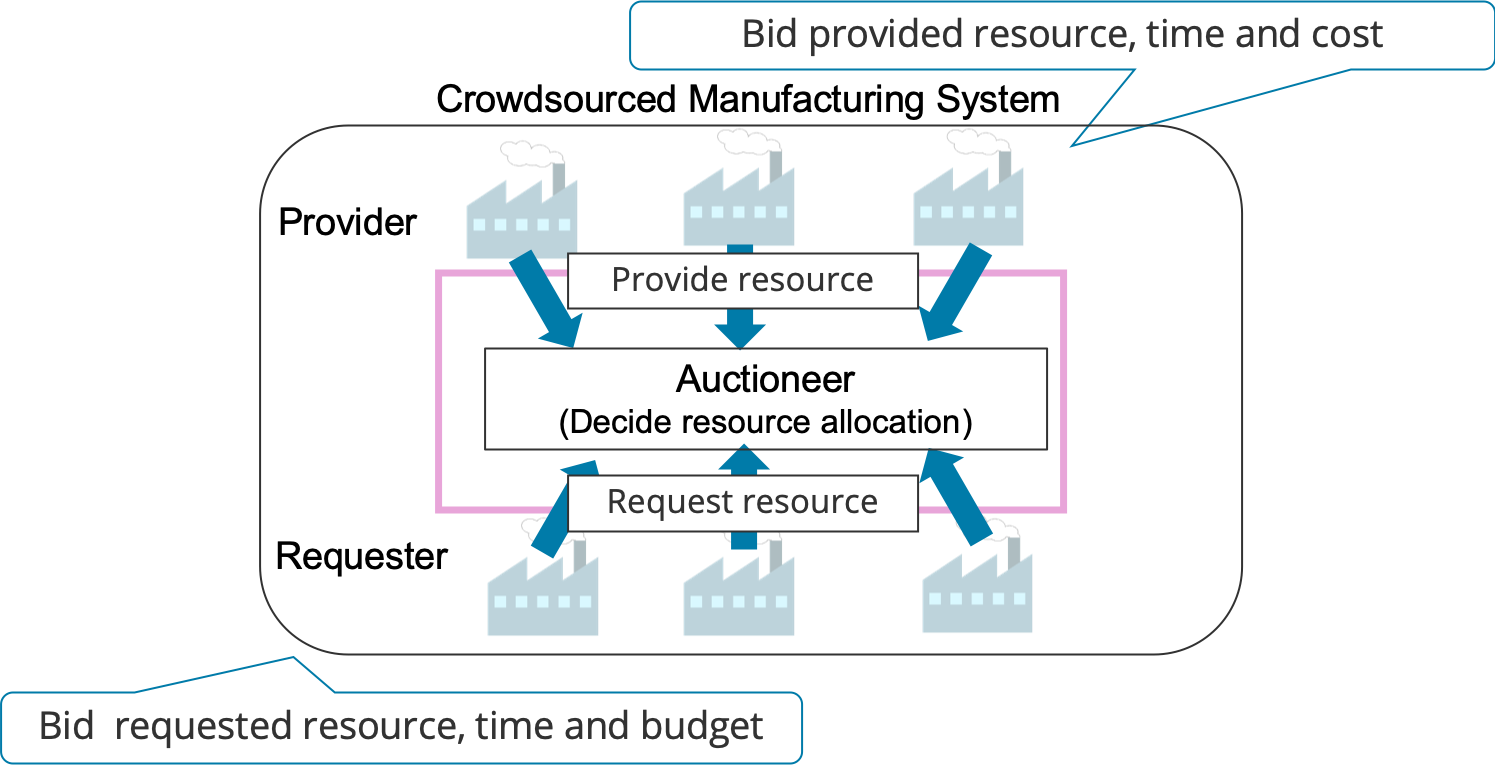
\includegraphics[width=0.6\textwidth,height=\textheight]{/Users/haradayoshiaki/Resarch/Paper/master-thesis/src/img/crowdsourced-manufacturing.png}
\caption{Crowedsourced Manufacturing}\label{fig:csmfg}
}
\end{figure}

リソースの提供側とリソースの要求側,そしてオークション主催者が存在する.それぞれの主体について説明する.

\begin{itemize}
\tightlist
\item
  リソース要求企業:要求するリソースの時間,予算を入札する.

  \begin{itemize}
  \tightlist
  \item
    予算はこの価格でリソースを使用すると利益が出ない価格とする.
  \end{itemize}
\item
  リソース提供企業:提供するリソースの時間,コストを入札する.

  \begin{itemize}
  \tightlist
  \item
    コストはこの価格でリソースの提供をしてしまうと利益が出ない値とする.
  \end{itemize}
\item
  オークション主催者:リソース提供・要求企業の入札を元にリソースの配分と,取引価格を決定する.

  \begin{itemize}
  \tightlist
  \item
    本研究においてはオークション主催者の利益は考慮しないものとする.
  \end{itemize}
\end{itemize}

\hypertarget{ux30aaux30fcux30afux30b7ux30e7ux30f3}{%
\section{オークション}\label{ux30aaux30fcux30afux30b7ux30e7ux30f3}}

本節ではオークションに関する一般的な説明を行った上で,本研究で行う組合せダブルオークションについて説明する.

\hypertarget{ux30aaux30fcux30afux30b7ux30e7ux30f3ux3068ux306f}{%
\subsection{オークションとは}\label{ux30aaux30fcux30afux30b7ux30e7ux30f3ux3068ux306f}}

オークションは,分散化された意思決定下において,財の配分と取引価格を決めるルールのことを指す\cite{market}.近年周波数帯オークション,ネット広告オークションでの成功から更に注目が集まっている\cite{yokoo}.

オークションの説明に使用される用語を以下に示す\cite{market}.

\begin{itemize}
\tightlist
\item
  財:オークションにおいて取引される資源のこと.
\item
  入札:財に対する評価値を表明すること.

  \begin{itemize}
  \tightlist
  \item
    この値を入札値と呼ぶ.
  \end{itemize}
\item
  準線形環境:金銭と効用(利益)が交換可能な環境のこと.

  \begin{itemize}
  \tightlist
  \item
    オークションではほどんどの場合で準線形環境を仮定する.
  \end{itemize}
\item
  買い手:金銭を払って財を入手することで利益を得たい主体のこと.

  \begin{itemize}
  \tightlist
  \item
    買い手の利益は財を入手するのに必要だった価格と評価値の差である.

    \begin{itemize}
    \tightlist
    \item
      例.評価値1000円の財を500円で買った買い手の利益は500円となる.
    \end{itemize}
  \end{itemize}
\item
  売り手:財を売って金銭を得ることで利益を得たい主体のこと.

  \begin{itemize}
  \tightlist
  \item
    売り手の利益は実際に受け取った報酬と評価値の差である.

    \begin{itemize}
    \tightlist
    \item
      例.評価値500円の財を1000円で売った売り手の利益は500円となる.
    \end{itemize}
  \end{itemize}
\item
  真の評価値:その値で財の取引を行うと,利益が0となる値のこと.
\item
  オークション主催者:ある目的を達成するために入札を元に財の配分と価格を決める主体のこと.

  \begin{itemize}
  \tightlist
  \item
    オークションの目的は参加者の効用の合計(社会的余剰)の最大,つまり総利益の最大となることが多い.
  \end{itemize}
\end{itemize}

\hypertarget{ux30aaux30fcux30afux30b7ux30e7ux30f3ux306eux8ca1ux306bux95a2ux3059ux308bux5206ux985e}{%
\subsection{オークションの財に関する分類}\label{ux30aaux30fcux30afux30b7ux30e7ux30f3ux306eux8ca1ux306bux95a2ux3059ux308bux5206ux985e}}

まずオークションに掛けられる財の種類による分類を説明する.

\hypertarget{ux5358ux4e00ux8ca1ux30aaux30fcux30afux30b7ux30e7ux30f3}{%
\subsubsection{単一財オークション}\label{ux5358ux4e00ux8ca1ux30aaux30fcux30afux30b7ux30e7ux30f3}}

オークションにかけられる財が1つであるオークションのことを単一財オークションと言う.

\hypertarget{ux8907ux6570ux8ca1ux30aaux30fcux30afux30b7ux30e7ux30f3}{%
\subsubsection{複数財オークション}\label{ux8907ux6570ux8ca1ux30aaux30fcux30afux30b7ux30e7ux30f3}}

オークションにかけられる財が複数財であるオークションのことを複数財オークションと言う.その中でもさらに複数ユニットオークションと組合せオークションの2つに分類される.

\hypertarget{ux8907ux6570ux30e6ux30cbux30c3ux30c8ux30aaux30fcux30afux30b7ux30e7ux30f3}{%
\paragraph{複数ユニットオークション}\label{ux8907ux6570ux30e6ux30cbux30c3ux30c8ux30aaux30fcux30afux30b7ux30e7ux30f3}}

同じ種類の財が複数単位かけられるオークションを複数ユニットオークションと言う.

\hypertarget{ux7d44ux5408ux305bux30aaux30fcux30afux30b7ux30e7ux30f3}{%
\paragraph{組合せオークション}\label{ux7d44ux5408ux305bux30aaux30fcux30afux30b7ux30e7ux30f3}}

複数種類の財が複数単位オークションにかけられ,入手できる組合せによって財の価値が変わるオークションを組合せオークションと言う.組合せオークションでは財の組合せに対して入札が可能である.組合せオークションでは,財同士の価値の間に依存関係がある場合が存在する.例えば,メモリとパソコンのように,メモリだけでは無価値で,またメモリが少ないPCが使い勝手が悪いと言うように,同時に所有できると価値が高まるなどの関係である.

\hypertarget{ux30aaux30fcux30afux30b7ux30e7ux30f3ux306eux5165ux672dux306bux95a2ux3059ux308bux5206ux985e}{%
\subsection{オークションの入札に関する分類}\label{ux30aaux30fcux30afux30b7ux30e7ux30f3ux306eux5165ux672dux306bux95a2ux3059ux308bux5206ux985e}}

次にオークションの入札を誰が行うかに着目した分類の説明を行う\cite{yokoo}.

\hypertarget{ux30b7ux30f3ux30b0ux30ebux30aaux30fcux30afux30b7ux30e7ux30f3ux30b7ux30f3ux30b0ux30ebux30b5ux30a4ux30c9ux30aaux30fcux30afux30b7ux30e7ux30f3}{%
\subsubsection{シングルオークション(シングルサイドオークション)}\label{ux30b7ux30f3ux30b0ux30ebux30aaux30fcux30afux30b7ux30e7ux30f3ux30b7ux30f3ux30b0ux30ebux30b5ux30a4ux30c9ux30aaux30fcux30afux30b7ux30e7ux30f3}}

入札を行う主体が買い手または売り手の片方である場合をシングルサイドオークションと言う.シングルサイドオークションの場合,入札者がオークション主催者の役割を担うことが多い.また売り手のみが入札を行うオークションを特にリバースオークションと呼ぶ場合もある.

\hypertarget{ux30c0ux30d6ux30ebux30aaux30fcux30afux30b7ux30e7ux30f3ux30c0ux30d6ux30ebux30b5ux30a4ux30c9ux30aaux30fcux30afux30b7ux30e7ux30f3}{%
\subsubsection{ダブルオークション(ダブルサイドオークション)}\label{ux30c0ux30d6ux30ebux30aaux30fcux30afux30b7ux30e7ux30f3ux30c0ux30d6ux30ebux30b5ux30a4ux30c9ux30aaux30fcux30afux30b7ux30e7ux30f3}}

入札を行う主体が買い手,売り手の双方である場合をダブルサイドオークションと言う.

\hypertarget{ux30aaux30fcux30afux30b7ux30e7ux30f3ux306eux8a55ux4fa1ux6307ux6a19}{%
\subsection{オークションの評価指標}\label{ux30aaux30fcux30afux30b7ux30e7ux30f3ux306eux8a55ux4fa1ux6307ux6a19}}

本節ではオークションが満たすべきとされる性質を説明する.

\hypertarget{ux500bux4ebaux5408ux7406ux6027}{%
\subsubsection{個人合理性}\label{ux500bux4ebaux5408ux7406ux6027}}

オークションに参加することで損をする者がいない性質を個人合理性と言う.個人合理性を満たさないオークションはオークションに参加することで損をしてしまう可能性があるので,参加者を集めることが極めて困難になる.

\hypertarget{ux30d1ux30ecux30fcux30c8ux52b9ux7387ux6027}{%
\subsubsection{パレート効率性}\label{ux30d1ux30ecux30fcux30c8ux52b9ux7387ux6027}}

誰かの効用を下げることに,他の誰かの効用を高めることができない状態をパレート効率的であると言う.そのような状態を導くオークションのことをパレート効率性を満たすオークションと言う.例えば,総利益が最大化されいる状態はパレート効率な状態であり,ある誰かの利益を下げない限り他の誰かの利益を上げることはできない.

\hypertarget{ux8010ux6226ux7565ux6027}{%
\subsubsection{耐戦略性}\label{ux8010ux6226ux7565ux6027}}

正直に真の評価値を申告することが支配戦略であるオークションを耐戦略性を満たすオークショと言う.つまり耐戦略性を満たすオークションでは.財に対する真の評価値をそのまま申告することが自分の利益を最大化する為の支配戦略となる.この性質を満たさないオークションは以下2点の欠点がある.

\begin{itemize}
\tightlist
\item
  オークション主催者が目指したい結果を正しく導くことができない

  \begin{itemize}
  \tightlist
  \item
    オークション主催者は入札者の評価値を元に財の配分を決める.しかし耐戦略性を満たさないオークションはその評価値が真の値とは限らず,導いた結果が本来の目的を達成できているかがわからない.
  \end{itemize}
\item
  入札者にとって使いづらいオークションになる

  \begin{itemize}
  \tightlist
  \item
    耐戦略性を満たさないオークションの場合正直な評価値の申告が支配戦略でないので,どのような評価値で入札するべきかを考える必要がある.
  \end{itemize}
\end{itemize}

\hypertarget{ux4ee3ux8868ux7684ux306aux30aaux30fcux30afux30b7ux30e7ux30f3ux306eux4f8b}{%
\subsection{代表的なオークションの例}\label{ux4ee3ux8868ux7684ux306aux30aaux30fcux30afux30b7ux30e7ux30f3ux306eux4f8b}}

本節では代表的なオークションについて説明する.

\hypertarget{ux30d5ux30a1ux30fcux30b9ux30c8ux30d7ux30e9ux30a4ux30b9ux30aaux30fcux30afux30b7ux30e7ux30f3}{%
\subsubsection{ファーストプライスオークション}\label{ux30d5ux30a1ux30fcux30b9ux30c8ux30d7ux30e9ux30a4ux30b9ux30aaux30fcux30afux30b7ux30e7ux30f3}}

ファーストプライスオークションは,勝者となった入札者の入札値で取引を行うオークションである.オークション主催者に対して利益を考慮した値を入札値として提出する.ファーストプライスオークションを以下に示す.

\begin{itemize}
\tightlist
\item
  ルール

  \begin{itemize}
  \tightlist
  \item
    財に対する入札を一度だけ行う.

    \begin{itemize}
    \tightlist
    \item
      入札値はオークション主催者にしか公開されない
    \end{itemize}
  \item
    一番入札値が高い入札者がその入札値でその財を得ることができる(リバースオークションの場合は一番低い入札値の入札者が売ることができる)
  \end{itemize}
\item
  分類

  \begin{itemize}
  \tightlist
  \item
    単一財オークション
  \item
    シングルサイドオークション
  \end{itemize}
\item
  性質

  \begin{itemize}
  \tightlist
  \item
    個人合理性○
  \item
    パレート効率性×
  \item
    耐戦略性×
  \end{itemize}
\end{itemize}

ファーストプライスオークションはオークションはルールがシンプルであり,また自分の入札値で取引が行われることから透明性が求められるネット広告オークションに使用される\cite{google}.しかし耐戦略性を満たせず,支配戦略が存在しないので,入札戦略が複雑になるなどのデメリットが存在する.

\hypertarget{ux30bbux30abux30f3ux30c9ux30d7ux30e9ux30a4ux30b9ux30aaux30fcux30afux30b7ux30e7ux30f3}{%
\subsubsection{セカンドプライスオークション}\label{ux30bbux30abux30f3ux30c9ux30d7ux30e9ux30a4ux30b9ux30aaux30fcux30afux30b7ux30e7ux30f3}}

セカンドプライスオークションは,単一財オークションであり,耐戦略性を満たすオークションである.勝者の取引価格は,このオークションで勝者として留まれる最小(最大)の価格となっている.またこの価格をcritiical
priceと呼ばれる.セカンドプライスオークションは以下の特徴を持つ.

\begin{itemize}
\tightlist
\item
  ルール

  \begin{itemize}
  \tightlist
  \item
    財に対する入札を一度だけ行う

    \begin{itemize}
    \tightlist
    \item
      入札値はオークション主催者にしか公開されない
    \end{itemize}
  \item
    一番入札値が高い入札者が勝者となり,その次に高い入札者の入札値(二位の価格)でその財を得ることができる(リバースオークションの場合は一番低い入札値の入札者が,その次に低い入札値で売ることができる)
  \end{itemize}
\item
  分類

  \begin{itemize}
  \tightlist
  \item
    単一財オークション
  \item
    シングルサイドオークション
  \end{itemize}
\item
  性質

  \begin{itemize}
  \tightlist
  \item
    個人合理性○
  \item
    パレート効率性○
  \item
    耐戦略性○
  \end{itemize}
\end{itemize}

セカンドプライスオークションは,二位の価格と財に対する真の評価値との差がオークションの勝者となった入札者の利益となる.このオークションは個人合理性・パレート効率性・耐戦略性を満たすことができる.現実の適用例としては,Yahooオークションなどが挙げられる\cite{yahoo}.

\hypertarget{ux30b6ux30e9ux30d0ux65b9ux5f0f}{%
\subsubsection{ザラバ方式}\label{ux30b6ux30e9ux30d0ux65b9ux5f0f}}

\begin{itemize}
\tightlist
\item
  \textbf{\emph{ダブルオークションの例として証券取引のザラバ方式を取り上げる...}}
\end{itemize}

\hypertarget{ux7d44ux5408ux305bux30c0ux30d6ux30ebux30aaux30fcux30afux30b7ux30e7ux30f3}{%
\section{組合せダブルオークション}\label{ux7d44ux5408ux305bux30c0ux30d6ux30ebux30aaux30fcux30afux30b7ux30e7ux30f3}}

本節では提案する2種類の組合せダブルオークションに基づいたリソース配分手法の共通部分について説明をする.

その準備としてまず,シングルサイド組合せオークションの代表的なオークションであるVCG(Vickrey--Clarke--Groves
Auction)オークション\cite{vickrey}について説明をする.

\hypertarget{vcgux30aaux30fcux30afux30b7ux30e7ux30f3vickreyclarkegroves-auction}{%
\subsubsection{VCGオークション(Vickrey--Clarke--Groves
Auction)}\label{vcgux30aaux30fcux30afux30b7ux30e7ux30f3vickreyclarkegroves-auction}}

VCGオークションはセカンドプライスオークションを一般化し,財の組合せに対する入札に対応したものである.理論的に優れた性質(個人合理性・パレート効率性・耐戦略性)を持つことからKing
of Mechanismsとも呼ばれる.VCGオークションは以下の特徴を持つ.

\begin{itemize}
\tightlist
\item
  ルール

  \begin{itemize}
  \tightlist
  \item
    財に対する入札を一度だけ行う.

    \begin{itemize}
    \tightlist
    \item
      入札値はオークション主催者にしか公開されない.
    \end{itemize}
  \item
    財の配分(オークションの勝者)は目的が総利益最大である組合せ最適化問題を解くことで決定される.

    \begin{itemize}
    \tightlist
    \item
      この問題を勝者決定問題と呼ぶ.
    \end{itemize}
  \item
    オークションの勝者は勝者として留まれる最小の価格を支払う.

    \begin{itemize}
    \tightlist
    \item
      価格を決める式は後述する.
    \end{itemize}
  \end{itemize}
\item
  分類

  \begin{itemize}
  \tightlist
  \item
    組合せオークション
  \item
    シングルサイドオークション
  \end{itemize}
\item
  性質

  \begin{itemize}
  \tightlist
  \item
    個人合理性○
  \item
    パレート効率性○
  \item
    耐戦略性○
  \end{itemize}
\end{itemize}

以下VCGオークション勝者決定問題,価格の決定方法にいついて詳しく説明し,その後で性質について詳しく説明する.ただし,買い手が入札の場合について説明する.

\hypertarget{ux52ddux8005ux6c7aux5b9aux554fux984cux306eux5b9aux5f0fux5316}{%
\paragraph{勝者決定問題の定式化}\label{ux52ddux8005ux6c7aux5b9aux554fux984cux306eux5b9aux5f0fux5316}}

VCGオークションの勝者を決める勝者決定問題は,組合せ最適化問題として定式化される.

定式化に用いる記号の定義は以下の通りである.

\begin{itemize}
\tightlist
\item
  \(j\): 買い手\(j\in \boldsymbol{J}\)
\item
  \(n\): 買い手\(j\)の入札\(n \in \boldsymbol{N}\)
\item
  \(f_{j,n}\):買い手\(j\)の\(n\)番目の入札の評価値
\item
  \(a_{j,n,r}\):買い手\(j\)の入札\(n\)に財\(r\)が含まれるとき1,含まれないとき0となる定数
\item
  \(r\):オークションにかけられる財\(r \in \boldsymbol{R}\)
\item
  \(V(\boldsymbol{J})\):提供企業の集合が\(\boldsymbol{J}\)であるときの勝者決定問題の目的関数値
\end{itemize}

上記の記号を用いて勝者決定問題を定式化する. \begin{align}
    {\rm max}\quad &V(\boldsymbol{J})=\sum_{j\in\boldsymbol{J}}\sum_{n \in \boldsymbol{N}}f_{j,n} \times x_{j,n}  \label{eq:vcg-obj}\\  
  {\rm s.t.} \quad &\sum_{j\in\boldsymbol{J}}\sum_{n\in\boldsymbol{N}} a_{j,n,r}\times x_{j,n}\leq 1 &(\forall r) \label{eq:vcg-cap-sub}\\
                  &\sum_{n \in \boldsymbol{N}} x_{j,n}\leq 1            &(\forall j)\\
                  &x_{j,n} \in \{0,1\}          &(\forall j,\forall n) 
\end{align}

決定変数は\(x_{j,n}\)であり,この値が1のとき入札者\(j\)の入札\(n\)が勝者となり入札に含れる財が落札され,この値が0のときに入札者\(j\)の入札\(n\)のは敗者となる.式\(\eqref{eq:vcg-obj}\)は目的関数であり,入札値の合計の最大化を表す.式\(\eqref{eq:vcg-cap-sub}\)は財を落札できるのは高々1入札者であることを表す制約である.これは財の容量制約を表す.

\hypertarget{ux4fa1ux683cux306eux5f0f}{%
\paragraph{価格の式}\label{ux4fa1ux683cux306eux5f0f}}

VCGオークションにおいて勝者となった\(j\)の入札\(n\)の支払い価格\(pay_{j}\)は以下のように定まる.
\begin{align}
pay_{j}  = -\{-f_{j,n}+V(\boldsymbol{J})\}+V(\boldsymbol{J}\backslash j)
\end{align}
\(V(\boldsymbol{J}\backslash j)\)は\(j\)を除いたオークションの勝者決定問題の目的関数値を表す.また,\(\{-f_{j,n}+V(\boldsymbol{J})\}\)は目的関数値から,支払いを決めようとする入札の入札値を除いた値である.よって\(pay_{j}\)は\(j\)の評価値に関わらず決定されている.

\hypertarget{ux6027ux8ceaux306eux8a3cux660e}{%
\paragraph{性質の証明}\label{ux6027ux8ceaux306eux8a3cux660e}}

\begin{itemize}
\tightlist
\item
  \textbf{\emph{VCGが耐戦略性や個人合理性を示すことを説明する}}
\end{itemize}

従来の製造業における組合せオークションを応用した研究では,シングルサイドオークションが多く扱われてきた\cite{suginouchi}.しかし本研究のクラウドソースドマニュファクチャリングにおいては.リソース提供企業・リソース要求企業の双方の意思を反映させる為に,ダブルオークションを適用する.そうすることで,提供企業と要求企業の総利益が最大化される配分を求めることを可能とした.本研究で行う組合せダブルオークションは以下の特徴を持つ.

\begin{itemize}
\tightlist
\item
  入札者

  \begin{itemize}
  \tightlist
  \item
    提供側

    \begin{itemize}
    \tightlist
    \item
      複数ユニットオークション

      \begin{itemize}
      \tightlist
      \item
        リソース複数単位(複数時間)提供することが可能である.
      \end{itemize}
    \end{itemize}
  \item
    要求側

    \begin{itemize}
    \tightlist
    \item
      組合せオークション

      \begin{itemize}
      \tightlist
      \item
        全てのリソースが揃わないと製品を作るが出来ず,利益を得ることが出来ないからである.
      \end{itemize}
    \end{itemize}
  \end{itemize}
\item
  オークションの目的

  \begin{itemize}
  \tightlist
  \item
    提供企業,要求企業の総利益の最大化とする.
  \end{itemize}
\end{itemize}

\hypertarget{ux5171ux901aux306eux6d41ux308c}{%
\section{共通の流れ}\label{ux5171ux901aux306eux6d41ux308c}}

提案するリソース配分手法は,大きく分けて入札作成部分と,オークション主催者のリソース配分と取引価格決定部分の2つからなる.

\begin{enumerate}
\def\labelenumi{\arabic{enumi}.}
\tightlist
\item
  入札作成

  \begin{itemize}
  \tightlist
  \item
    リソース提供企業はオークション主催者に入札を行う.

    \begin{itemize}
    \tightlist
    \item
      \textbf{\emph{文字を使ってどのような入札を作成するかを説明する...}}
    \end{itemize}
  \item
    リソース提供企業はオークション主催者に入札を行う.

    \begin{itemize}
    \tightlist
    \item
      \textbf{\emph{文字を使ってどのような入札を作成するかを説明する...}}
    \end{itemize}
  \end{itemize}
\item
  オークション主催者はリソースの配分と,取引価格の決定する.
\end{enumerate}

\hypertarget{ux5165ux672dux4f5cux6210}{%
\subsection{入札作成}\label{ux5165ux672dux4f5cux6210}}

2の部分の具体的なアルゴリズムは次章以降で説明する.ここでは1の入札作成について例を用いて説明する.

\begin{itemize}
\tightlist
\item
  \textbf{\emph{図を使い入札の例を示す...}}
\end{itemize}

\hypertarget{ux8a55ux4fa1ux6307ux6a19}{%
\subsection{評価指標}\label{ux8a55ux4fa1ux6307ux6a19}}

本研究で提案するリソース配分手法の評価指標について述べる.オークションの観点の評価指標は以下の2つである.

\begin{itemize}
\tightlist
\item
  パレート効率性

  \begin{itemize}
  \tightlist
  \item
    総利益の値を評価する.
  \end{itemize}
\item
  耐戦略性

  \begin{itemize}
  \tightlist
  \item
    虚偽申告を行ったある1企業の利益を評価する.
  \end{itemize}
\end{itemize}

クラウドソースドマニュファクチャリングの観点の評価指標は以下の6つとする.

\begin{itemize}
\tightlist
\item
  総提供企業利益

  \begin{itemize}
  \tightlist
  \item
    提供企業の利益の合計を評価する.
  \end{itemize}
\item
  総要求企業利益

  \begin{itemize}
  \tightlist
  \item
    要求企業の利益の合計を評価する.
  \end{itemize}
\item
  1提供企業利益
\item
  1要求企業利益
\item
  提供企業の稼働率の変化

  \begin{itemize}
  \tightlist
  \item
    リソースを提供する前と提供した後での稼働率の増加分について評価する.
  \end{itemize}
\item
  勝者となった要求の割合

  \begin{itemize}
  \tightlist
  \item
    全要求企業の内,勝者となった要求の割合について評価する.
  \end{itemize}
\end{itemize}

次章以降では,以上の評価指標を用いて手法I:パレート効率性を満たす手法・手法II:耐戦略性を満たす手法の特性を評価する.

\hypertarget{ux7d50ux8a00}{%
\section{結言}\label{ux7d50ux8a00}}

\begin{itemize}
\tightlist
\item
  \textbf{\emph{結言を述べる...}}
\end{itemize}

\hypertarget{ux624bux6cd5iux30d1ux30ecux30fcux30c8ux52b9ux7387ux6027ux3092ux6e80ux305fux3059ux624bux6cd5}{%
\chapter{手法I:パレート効率性を満たす手法}\label{ux624bux6cd5iux30d1ux30ecux30fcux30c8ux52b9ux7387ux6027ux3092ux6e80ux305fux3059ux624bux6cd5}}

\hypertarget{ux30a2ux30ebux30b4ux30eaux30baux30e0}{%
\section{アルゴリズム}\label{ux30a2ux30ebux30b4ux30eaux30baux30e0}}

手法I:パレート効率性を満たす手法のアルゴリズムについて説明する.

\hypertarget{ux6982ux8981}{%
\subsection{概要}\label{ux6982ux8981}}

以下に本手法のアルゴリズムの流れを示す.

\begin{enumerate}
\def\labelenumi{\arabic{enumi}.}
\tightlist
\item
  入札作成

  \begin{itemize}
  \item
    リソース提供企業はオークション主催者に対して,入札を作成する.
  \item
    リソース要求企業はオークション主催者に対して,入札を作成する.
  \end{itemize}
\item
  オークション主催者は,入札を元に勝者決定問題を解くことでリソース配分を決定する.
\item
  オークション主催者は,リソースの取引価格を決定する.
\end{enumerate}

1に関しては,前節の入札を作成をし,2,3について次節以降で説明する.説明に使用する記号の定義を以下に示す.

\begin{itemize}
\tightlist
\item
  \(i\):リソース提供企業(\(i \in \boldsymbol{I}\))
\item
  \(j\): リソース要求企業(\(j \in \boldsymbol{J}\))
\item
  \(r\):オークションにかけられるリソース(\(r \in \boldsymbol{R}\))
\item
  \(c_{i,r}\):提供企業\(i\)が提供するリソース\(r\)のコスト
\item
  \(TP_{i,r}\):提供企業\(i\)がリソース\(r\)を提供する時間
\item
  \(n\): 要求企業\(j\)の入札(\(n \in \boldsymbol{N}\))
\item
  \(v_{j,n}\):要求企業\(j\)の\(n\)番目の入札の評価値
\item
  \(TR_{j,n.r}\):要求企業\(j\)の\(n\)番目の入札においてリソース\(r\)を要求する時間
\item
  \(P(\boldsymbol{I},\boldsymbol{J})\):提供企業の集合が\(\boldsymbol{J}\),要求企業の集合\(\boldsymbol{J}\)であるときの勝者決定問題
\item
  \(V(\boldsymbol{I},\boldsymbol{J})\):問題\(P(\boldsymbol{I},\boldsymbol{J})\)の目的関数値
\item
  \(trade_{i,r,j,n}\):提供企業\(i\)が要求企業\(j\)の勝者となった入札\(n\)に対してリソース\(r\)を\(x_{i,r,j,n}\){[}Ts{]}提供するときの取引価格
\item
  \(sumTR_{j,n,r}\):要求企業\(j\)が入札\(n\)におけるリソース要求時間の合計
\end{itemize}

\hypertarget{ux30eaux30bdux30fcux30b9ux914dux5206ux306eux6c7aux5b9a}{%
\subsection{\texorpdfstring{リソース配分の決定
\label{method1-resorce}}{リソース配分の決定 }}\label{ux30eaux30bdux30fcux30b9ux914dux5206ux306eux6c7aux5b9a}}

リソースの配分を決める勝者決定問題\(P(\boldsymbol{I},\boldsymbol{J})\)は組合せ最適化問題として定式化される.以下にその定式化を示す.

\begin{align}
  {\rm max}\quad  V(\boldsymbol{I},\boldsymbol{J})=&\sum_{j\in \boldsymbol{J}}\sum_{n\in\boldsymbol{N}}v_{j} \times y_{j,n} - \sum_{i\in\boldsymbol{I}}\sum_{r\in\boldsymbol{R}}\sum_{j\in\boldsymbol{J}}\sum_{n\in\boldsymbol{N}}c_{i,r} \times x_{i,r,j,n} \label{pij-obj}\\
    {\rm s.t.} \quad &\sum_{j\in \boldsymbol{J}}\sum_{n\in\boldsymbol{N}}x_{i,r,j,n} \leq TP_{i,r} \quad (\forall i, \forall r) \label{pij-subto-cap}\\
  &\begin{cases}
    x_{i,r,j,n} = 0 \quad (\forall i, \forall r)&({\rm if} \ y_{j,n}=0) \\
    \sum_{j \in \boldsymbol{J}}\sum_{n\in\boldsymbol{N}} TR_{j,n,r} \times x_{i,r,j,n} = TR_{j,n,r}
    \quad  (\forall i, \forall r)&({\rm if} \ y_{j,n}=1) 
  \end{cases}\label{pij-subto-bundle}\\
    &\sum_{n\in \boldsymbol{N}}y_{j,n}  \leq 1 \quad (\forall j) \label{pij-subto-1winner}\\
    &x_{i,r,j,n} \in \boldsymbol{Z}\label{pij-decision-x}\\
    &y_{j,n} \in {0,1} \label{pij-decision-y}
\end{align}

決定変数は\(x_{i,r,j,n}\)と\(y_{j,n}\)である.\(x_{i,r,j,n}\)は企業\(i\)と企業\(j\)がリソース\(r\)を取引する量を表す整数変数であり,\(y_{j,n}\)は企業\(j\)の入札\(n\)が選ばれるとき1,選ばれない時0となる変数である.式\(\eqref{pij-obj}\)は目的関数であり,総利益最大化を表す.式\(\eqref{pij-subto-cap}\)は提供企業のリソースの容量制約を表す.式\(\eqref{pij-subto-bundle}\)は組合せ入札に関する制約であり,要求企業\(j\)の入札\(n\)が選ばれないときは,どのリソース要求も満たさないための制約,要求企業\(j\)の入札\(n\)が選ばれるときは,その入札のリソース要求を全て満たすための制約である.式\(\eqref{pij-subto-1winner}\)は勝者となる要求企業の入札は高々1つとする制約である.この組合せ最適化問題を解くことで勝者となる要求企業の入札と,それに対する提供リソースの配分を決定する.また,問題\(P(\boldsymbol{I},\boldsymbol{J})\)の最適解は総利益が最大化されているので,パレート効率な状態となっている.

\hypertarget{ux53d6ux5f15ux4fa1ux683cux6c7aux5b9a}{%
\subsection{取引価格決定}\label{ux53d6ux5f15ux4fa1ux683cux6c7aux5b9a}}

前節のリソース配分を元に取引価格\(trade_{i,r,j,n}\)を決定する.手法Iの取引価格はお互いの評価値の平均の価格から決定され,以下の式で表される.
\begin{align}
trade_{i,r,j,n}=&\frac{c_{i,r}+\{v_{j,n}×\frac{TR_{j,n,r}}{sumTR_{j,n}}/TR_{j,n,r}\}}{2}\times x_{i,r,j,n} \label{1-trade}\\
sumTR_{j,n} = &\sum_{r  \in R} TR_{j,n,r} \label{sumtime}
\end{align}
\(sumTR_{j,n,r}\)は要求企業\(j\)が入札\(n\)におけるリソース要求時間の合計である.よって式\(\eqref{1-trade}\)の\(v_{j,n}×\frac{TR_{j,n,r}}{sumTR_{j,n}}/TR_{j,n,r}\)はリソース\(r\)の1{[}Ts{]}分の予算を表す.従って式\(\eqref{1-trade}\)はお互いの評価値の平均で取引を行っていることとなる.

\hypertarget{ux7279ux5fb4}{%
\subsection{特徴}\label{ux7279ux5fb4}}

手法Iは問題\(P(\boldsymbol{I},\boldsymbol{J})\)の最適解に従いリソースの配分を決めるので,パレート効率な配分が実現される.しかし取引価格は,お互いの評価値の平均をとるので,この価格は提供企業,要求企業ともにcritical
priceとなっておらず耐戦略性を満たすことはできない.ただし同じような評価値を持つ企業が増加した場合,虚偽申告を行うと,オークションの敗者になる可能性が高くなる.従って同じような評価値を持つ企業が増加するほど正直な申告が支配戦略になっていく.

\hypertarget{ux7279ux6027ux8a55ux4fa1}{%
\section{特性評価}\label{ux7279ux6027ux8a55ux4fa1}}

本節では計算機実験により手法Iの特性を評価する.問題\(P(\boldsymbol{I},\boldsymbol{J})\)の求解には数理計画ソルバーCPLEXを用いる.共通の実験条件を以下に示す.ただし{[}min,
max{]}はminからmaxの一様乱数とする.

\begin{itemize}
\tightlist
\item
  提供企業\(|\boldsymbol{J}|=25\)

  \begin{itemize}
  \tightlist
  \item
    各企業2種類のリソースを遊休時間に提供する
  \item
    遊休時間\(TP_{i,r}\) {[}Ts{]}を{[}100, 200{]}で決定する
  \item
    コスト\(c_{i,r}\)は{[}2.0, 4.0{]} {[}円{]}とする
  \end{itemize}
\item
  要求企業\(|\boldsymbol{I}|=10\)

  \begin{itemize}
  \tightlist
  \item
    各企業\(|\boldsymbol{N}|\)=3個の入札を作成
  \item
    R種類のリソースを各 {[}0, 200{]} {[}Ts{]}要求する
  \item
    予算\(v_{j,n}\)は合計要求時間と重み{[}3.0, 5.0{]}の積{[}円{]}とする
  \end{itemize}
\end{itemize}

\hypertarget{ux63d0ux4f9bux4f01ux696dux306eux865aux507dux7533ux544aux7387ux306eux5909ux66f4}{%
\subsection{1提供企業の虚偽申告率の変更}\label{ux63d0ux4f9bux4f01ux696dux306eux865aux507dux7533ux544aux7387ux306eux5909ux66f4}}

本節では1提供企業の虚偽申告率を変更する実験を行う.手法Iは耐戦略性を満たせず,虚偽申告により利益を高められることを確認する.ここでの虚偽申告率とは,コストにある割合分上乗して入札値として申告するとした際の,その割合のことを指す.例えば,コストが10円,虚偽申告率が10\%の場合は11円と入札する.コストをふっかけることで利益を上げようとする企業を想定している.

以下に本実験における実験条件を示す.

\begin{itemize}
\tightlist
\item
  1提供企業の虚偽申告率:0\%,10\%,20\%,30\%

  \begin{itemize}
  \tightlist
  \item
    虚偽申告が0\%のときは正直にコストを申告する.
  \end{itemize}
\item
  試行回数:1回
\end{itemize}

\hypertarget{ux5b9fux9a13ux7d50ux679c}{%
\subsubsection{実験結果}\label{ux5b9fux9a13ux7d50ux679c}}

Table~\ref{tbl:m1-1-total-profit}-Table~\ref{tbl:m1-1-false-requester-total-profit}は,それぞれ総利益,総提供企業利益,総要求企業利益,虚偽申告を行った1提供企業の利益を示す.

\hypertarget{tbl:m1-1-total-profit}{}
\begin{longtable}[H]{@{}lllll@{}}
\caption{\label{tbl:m1-1-total-profit}Total Profit in Method 1: A
provider report false cost}\tabularnewline
\toprule
False reporting rate & 0\% & 10\% & 20\% & 30\%\tabularnewline
\midrule
\endfirsthead
\toprule
False reporting rate & 0\% & 10\% & 20\% & 30\%\tabularnewline
\midrule
\endhead
Total Profit & 9175.28 & 9175.22 & 9175.22 & 9049.41\tabularnewline
\bottomrule
\end{longtable}

\hypertarget{tbl:m1-1-providers-total-profit}{}
\begin{longtable}[H]{@{}lllll@{}}
\caption{\label{tbl:m1-1-providers-total-profit}Providers Total Profit:
in Method 1: A provider report false cost}\tabularnewline
\toprule
False reporting rate & 0\% & 10\% & 20\% & 30\%\tabularnewline
\midrule
\endfirsthead
\toprule
False reporting rate & 0\% & 10\% & 20\% & 30\%\tabularnewline
\midrule
\endhead
Providers Total Profit & 4587.64 & 4613.49 & 4639.38 &
4524.70\tabularnewline
\bottomrule
\end{longtable}

\hypertarget{tbl:m1-1-requesters-total-profit}{}
\begin{longtable}[H]{@{}lllll@{}}
\caption{\label{tbl:m1-1-requesters-total-profit}Requesters Total Profit
in Method 1:A provider report false cost}\tabularnewline
\toprule
False reporting rate & 0\% & 10\% & 20\% & 30\%\tabularnewline
\midrule
\endfirsthead
\toprule
False reporting rate & 0\% & 10\% & 20\% & 30\%\tabularnewline
\midrule
\endhead
Requesters Total Profit & 4587.64 & 4561.72 & 4535.84 &
4524.70\tabularnewline
\bottomrule
\end{longtable}

\hypertarget{tbl:m1-1-false-requester-total-profit}{}
\begin{longtable}[H]{@{}lllll@{}}
\caption{\label{tbl:m1-1-false-requester-total-profit}False reporting
Requester Profit in Method 1: A provider report false
cost}\tabularnewline
\toprule
False reporting rate & 0\% & 10\% & 20\% & 30\%\tabularnewline
\midrule
\endfirsthead
\toprule
False reporting rate & 0\% & 10\% & 20\% & 30\%\tabularnewline
\midrule
\endhead
Requester Profit & 112.47 & 139.30 & 227.77 & 0\tabularnewline
\bottomrule
\end{longtable}

\hypertarget{ux8003ux5bdf}{%
\subsubsection{考察}\label{ux8003ux5bdf}}

Table~\ref{tbl:m1-1-false-requester-total-profit}において,虚偽申告率が20\%まで利益が増加している.20\%から30\%にかけて利益が下がったのは,申告したコストが高くなり,リソースの配分が変わり,オークションにおいて勝者となることができなくなってしまったからだと考える.よってオークションの敗者になるまで,虚偽申告を行うことで利益を上げることが可能なことがわかり,耐戦略性を満たすことができないことが確認できる.またTable~\ref{tbl:m1-1-total-profit}の虚偽申告率0から20\%総利益があまり変化がないにも関わらず,Table~\ref{tbl:m1-1-providers-total-profit}の総提供企業利益が増加し,Table~\ref{tbl:m1-1-requesters-total-profit}の総要求企業利益が減少している.従って虚偽申告により,利益が提供企業に移転していることが確認できる.

\hypertarget{ux8981ux6c42ux4f01ux696dux306eux865aux507dux7533ux544aux7387ux306eux5909ux66f4}{%
\subsection{1要求企業の虚偽申告率の変更}\label{ux8981ux6c42ux4f01ux696dux306eux865aux507dux7533ux544aux7387ux306eux5909ux66f4}}

本節では1要求企業の虚偽申告率を変更する実験を行う.手法Iは耐戦略性を満たせず,虚偽申告により利益を高められることを確認する.ここでの虚偽申告率は,入札の予算に対して減額する割合とする.例えば,虚偽申告率が10\%のときは,予算が1000円の入札を900円と申告する.予算を過少申告することで,より安い価格でリソースを入手しようとする企業を想定する.

以下に本実験における実験条件を示す.

\begin{itemize}
\tightlist
\item
  1要求企業の虚偽申告率:0\%,10\%,20\%,30\%

  \begin{itemize}
  \tightlist
  \item
    虚偽申告が0\%のときは正直に予算を申告する.
  \end{itemize}
\item
  試行回数:1回
\end{itemize}

\hypertarget{ux7d50ux679c}{%
\subsubsection{結果}\label{ux7d50ux679c}}

Table~\ref{tbl:m1-2-total-profit}-Table~\ref{tbl:m1-2-false-requester-profit}は,それぞれ総利益,総提供企業利益,総要求企業利益,虚偽申告を行った1要求企業の利益を示す.

\hypertarget{tbl:m1-2-total-profit}{}
\begin{longtable}[H]{@{}lllll@{}}
\caption{\label{tbl:m1-2-total-profit}Total Profit in Method 1: A
requester report false budget}\tabularnewline
\toprule
False reporting rate & 0\% & 10\% & 20\% & 30\%\tabularnewline
\midrule
\endfirsthead
\toprule
False reporting rate & 0\% & 10\% & 20\% & 30\%\tabularnewline
\midrule
\endhead
Total Profit & 9175.28 & 9175.28 & 9175.28 & 9175.28\tabularnewline
\bottomrule
\end{longtable}

\hypertarget{tbl:m1-2-providers-total-profit}{}
\begin{longtable}[H]{@{}lllll@{}}
\caption{\label{tbl:m1-2-providers-total-profit}Total Providers Profit
in Method 1: A requester report false budget}\tabularnewline
\toprule
False reporting rate & 0\% & 10\% & 20\% & 30\%\tabularnewline
\midrule
\endfirsthead
\toprule
False reporting rate & 0\% & 10\% & 20\% & 30\%\tabularnewline
\midrule
\endhead
Providers Total Profit & 4587.64 & 4492.88 & 4398.11 &
4303.35\tabularnewline
\bottomrule
\end{longtable}

\hypertarget{tbl:m1-2-requesters-total-profit}{}
\begin{longtable}[H]{@{}lllll@{}}
\caption{\label{tbl:m1-2-requesters-total-profit}Total Providers Profit
in Method 1: A requester report false budget}\tabularnewline
\toprule
False reporting rate & 0\% & 10\% & 20\% & 30\%\tabularnewline
\midrule
\endfirsthead
\toprule
False reporting rate & 0\% & 10\% & 20\% & 30\%\tabularnewline
\midrule
\endhead
Requesters Total Profit & 4587.64 & 4682.41 & 4777.17 &
4871.93\tabularnewline
\bottomrule
\end{longtable}

\hypertarget{tbl:m1-2-false-requester-profit}{}
\begin{longtable}[H]{@{}lllll@{}}
\caption{\label{tbl:m1-2-false-requester-profit}Total Providers Profit
in Method 1: A requester report false budget}\tabularnewline
\toprule
False reporting rate & 0\% & 10\% & 20\% & 30\%\tabularnewline
\midrule
\endfirsthead
\toprule
False reporting rate & 0\% & 10\% & 20\% & 30\%\tabularnewline
\midrule
\endhead
Provider Profit & 412.8505 & 457.5463 & 573.548 &
694.5275\tabularnewline
\bottomrule
\end{longtable}

\hypertarget{ux8003ux5bdf-1}{%
\subsubsection{考察}\label{ux8003ux5bdf-1}}

Table~\ref{tbl:m1-2-false-requester-profit}より,申告率が増加するごとに利益が上がっていることが確認できる.よって手法Iが耐戦略性を満たせないことが確認できる.またTable~\ref{tbl:m1-2-total-profit}において,総利益は変化がないが,Table~\ref{tbl:m1-2-providers-total-profit}の提供企業利益は減少し,Table~\ref{tbl:m1-2-requesters-total-profit}の総要求企業利益は増加している,これより提供側に利益が移転していることがわかる.

\hypertarget{ux63d0ux4f9bux5074ux304cux7533ux544aux3059ux308bux30b3ux30b9ux30c8ux306eux5e45ux306eux5909ux66f4}{%
\subsection{提供側が申告するコストの幅の変更}\label{ux63d0ux4f9bux5074ux304cux7533ux544aux3059ux308bux30b3ux30b9ux30c8ux306eux5e45ux306eux5909ux66f4}}

本節では,提供側が申告するコストの幅を変更する実験を行う.幅を変更したそれぞれの場合において,ある提供企業が虚偽申告率を変更した場合に利益がどのように変化するかを確認する.各企業が申告するコストの幅が狭くなる,つまり同じようなコストの企業が集まると正直な申告が支配戦略になることを確認する.

\begin{itemize}
\tightlist
\item
  コストを発生させる乱数の幅:2.5,2.0,1.5,1.0

  \begin{itemize}
  \tightlist
  \item
    コストを{[}1.75,4.25{]},{[}2.0,4.0{]},{[}2.25,3.75{]},{[}2.5,3.5{]}で生成する.
  \end{itemize}
\item
  試行回数:10回
\end{itemize}

\hypertarget{ux5b9fux9a13ux7d50ux679c-1}{%
\subsubsection{実験結果}\label{ux5b9fux9a13ux7d50ux679c-1}}

Table~\ref{tbl:m1-3-2.5-false-provider-profit}-Table~\ref{tbl:m1-3-1.0-false-provider-profit}は,それぞれコストの幅が2.5,2.0,1.5,1.0のときの虚偽申告提供企業の利益を表す.

\hypertarget{tbl:m1-3-2.5-false-provider-profit}{}
\begin{longtable}[H]{@{}lllll@{}}
\caption{\label{tbl:m1-3-2.5-false-provider-profit}False reporting
Provider Profit in Method 1:cost range=2.5}\tabularnewline
\toprule
False reporting rate & 0\% & 10\% & 20\% & 30\%\tabularnewline
\midrule
\endfirsthead
\toprule
False reporting rate & 0\% & 10\% & 20\% & 30\%\tabularnewline
\midrule
\endhead
AVE. & 173.07 & 194.66 & 184.64 & 143.98\tabularnewline
S.D. & 97.60 & 104.51 & 124.04 & 124.09\tabularnewline
\bottomrule
\end{longtable}

\hypertarget{tbl:m1-3-2.0-false-provider-profit}{}
\begin{longtable}[H]{@{}lllll@{}}
\caption{\label{tbl:m1-3-2.0-false-provider-profit}False reporting
Provider Profit in Method 1:cost range=2.0}\tabularnewline
\toprule
False reporting rate & 0\% & 10\% & 20\% & 30\%\tabularnewline
\midrule
\endfirsthead
\toprule
False reporting rate & 0\% & 10\% & 20\% & 30\%\tabularnewline
\midrule
\endhead
AVE. & 189.28 & 203.53 & 201.61 & 172.39\tabularnewline
S.D. & 105.08 & 103.87 & 79.45 & 88.61\tabularnewline
\bottomrule
\end{longtable}

\hypertarget{tbl:m1-3-1.5-false-provider-profit}{}
\begin{longtable}[H]{@{}lllll@{}}
\caption{\label{tbl:m1-3-1.5-false-provider-profit}False reporting
Provider Profit in Method 1:cost range=1.5}\tabularnewline
\toprule
False reporting rate & 0\% & 10\% & 20\% & 30\%\tabularnewline
\midrule
\endfirsthead
\toprule
False reporting rate & 0\% & 10\% & 20\% & 30\%\tabularnewline
\midrule
\endhead
AVE. & 208.02 & 209.98 & 158.56 & 84.83\tabularnewline
S.D. & 89.21 & 116.48 & 125.35 & 88.38\tabularnewline
\bottomrule
\end{longtable}

\hypertarget{tbl:m1-3-1.0-false-provider-profit}{}
\begin{longtable}[H]{@{}lllll@{}}
\caption{\label{tbl:m1-3-1.0-false-provider-profit}False reporting
Provider Profit in Method 1:cost range=1.0}\tabularnewline
\toprule
False reporting rate & 0\% & 10\% & 20\% & 30\%\tabularnewline
\midrule
\endfirsthead
\toprule
False reporting rate & 0\% & 10\% & 20\% & 30\%\tabularnewline
\midrule
\endhead
AVE. & 165.03 & 147.50 & 75.35 & 60.80\tabularnewline
S.D. & 89.19 & 90.53 & 94.68 & 69.13\tabularnewline
\bottomrule
\end{longtable}

Table~\ref{tbl:m1-3-2.5-false-provider-profit}-Table~\ref{tbl:m1-3-1.0-false-provider-profit}の結果を,正直にコストを申告した場合に対して虚偽申告を行った際の利益率の表に直したものをTable~\ref{tbl:m1-3-profit-rate}に示す.

\hypertarget{tbl:m1-3-profit-rate}{}
\begin{longtable}[H]{@{}llll@{}}
\caption{\label{tbl:m1-3-profit-rate}Ratio of increased profit to the
Profits for reporting truthful cost}\tabularnewline
\toprule
False reporting rate & 10\% & 20\% & 30\%\tabularnewline
\midrule
\endfirsthead
\toprule
False reporting rate & 10\% & 20\% & 30\%\tabularnewline
\midrule
\endhead
cost range=2.5 & 12.5\% & 6.7\% & -16.8\%\tabularnewline
cost range=2.0 & 7.5\% & 6.5\% & -6.1\%\tabularnewline
cost range=1.5 & 0.9\% & -23.8\% & -59.2\%\tabularnewline
cost range=1.0 & -10.6\% & -54.3\% & -63.2\%\tabularnewline
\bottomrule
\end{longtable}

\hypertarget{ux8003ux5bdf-2}{%
\subsubsection{考察}\label{ux8003ux5bdf-2}}

Table~\ref{tbl:m1-3-profit-rate}より,コストの幅が2.5のときは虚偽申告率が20\%のときまで利益が増加しているが,コストの幅が1.5のときは利益が減少している.またコストの幅が1.0のときは,10\%の虚偽申告でも利益が減少しており,コストの幅が狭くなるごとに正直な申告が支配戦略に近づくことがわかる.

\hypertarget{ux8981ux6c42ux4f01ux696dux304cux7533ux544aux3059ux308bux4e88ux7b97ux306eux5e45ux306eux5909ux66f4}{%
\subsection{要求企業が申告する予算の幅の変更}\label{ux8981ux6c42ux4f01ux696dux304cux7533ux544aux3059ux308bux4e88ux7b97ux306eux5e45ux306eux5909ux66f4}}

本節では,提供側が申告する予算の幅を変更する実験を行う.幅を変更したそれぞれの場合において,ある要求企業が虚偽申告率を変更した場合に利益がどのように変化するかを確認する.前節と同様に,同じような予算の企業が集まると正直な申告が支配戦略になることを確認する.

\begin{itemize}
\tightlist
\item
  コストを発生させる乱数の幅:2.5,2.0,1.5,1.0

  \begin{itemize}
  \tightlist
  \item
    コストを{[}2.75,5.25{]},{[}3.0,5.0{]},{[}3.25,4.75{]},{[}3.5,4.5{]}で生成する.
  \end{itemize}
\item
  試行回数:10回
\end{itemize}

\hypertarget{ux5b9fux9a13ux7d50ux679c-2}{%
\subsubsection{実験結果}\label{ux5b9fux9a13ux7d50ux679c-2}}

Table~\ref{tbl:m1-4-2.5-requester-profit}-Table~\ref{tbl:m1-4-1.0-requester-profit}は,それぞれ予算の幅が2.5,2.0,1.5,1.0のときの虚偽申告要求企業の利益を表す.

\hypertarget{tbl:m1-4-2.5-requester-profit}{}
\begin{longtable}[H]{@{}lllll@{}}
\caption{\label{tbl:m1-4-2.5-requester-profit}False reporting Requester
Profit in Method 1:budget range=2.5}\tabularnewline
\toprule
False reporting rate & 0\% & 10\% & 20\% & 30\%\tabularnewline
\midrule
\endfirsthead
\toprule
False reporting rate & 0\% & 10\% & 20\% & 30\%\tabularnewline
\midrule
\endhead
AVE. & 408.94 & 448.28 & 453.20 & 230.52\tabularnewline
S.D. & 293.34 & 376.17 & 477.45 & 466.90\tabularnewline
\bottomrule
\end{longtable}

\hypertarget{tbl:m1-4-2.0-requester-profit}{}
\begin{longtable}[H]{@{}lllll@{}}
\caption{\label{tbl:m1-4-2.0-requester-profit}False reporting Requester
Profit in Method 1:budget range=2.0}\tabularnewline
\toprule
False reporting rate & 0\% & 10\% & 20\% & 30\%\tabularnewline
\midrule
\endfirsthead
\toprule
False reporting rate & 0\% & 10\% & 20\% & 30\%\tabularnewline
\midrule
\endhead
AVE. & 355.23 & 398.52 & 291.70 & 171.81\tabularnewline
S.D. & 244.25 & 354.22 & 366.58 & 351.41\tabularnewline
\bottomrule
\end{longtable}

\hypertarget{tbl:m1-4ux20131.5-requester-profit}{}
\begin{longtable}[H]{@{}lllll@{}}
\caption{\label{tbl:m1-4ux20131.5-requester-profit}False reporting
Requester Profit in Method 1:budget range=1.5}\tabularnewline
\toprule
False reporting rate & 0\% & 10\% & 20\% & 30\%\tabularnewline
\midrule
\endfirsthead
\toprule
False reporting rate & 0\% & 10\% & 20\% & 30\%\tabularnewline
\midrule
\endhead
AVE. & 329.75 & 249.590 & 123.20 & 0\tabularnewline
S.D. & 231.12 & 256.35 & 246.64 & 0\tabularnewline
\bottomrule
\end{longtable}

\hypertarget{tbl:m1-4-1.0-requester-profit}{}
\begin{longtable}[H]{@{}lllll@{}}
\caption{\label{tbl:m1-4-1.0-requester-profit}False reporting Requester
Profit in Method 1:budget range=1.0}\tabularnewline
\toprule
False reporting rate & 0\% & 10\% & 20\% & 30\%\tabularnewline
\midrule
\endfirsthead
\toprule
False reporting rate & 0\% & 10\% & 20\% & 30\%\tabularnewline
\midrule
\endhead
AVE. & 433.00 & 306.62 & 220.93 & 0\tabularnewline
S.D. & 159.78 & 317.43 & 352.38 & 0\tabularnewline
\bottomrule
\end{longtable}

Table~\ref{tbl:m1-4-2.5-requester-profit}-Table~\ref{tbl:m1-4-1.0-requester-profit}の結果を,正直にコストを申告した場合に対して虚偽申告を行った際の利益率の表に直したものをTable~\ref{tbl:m1-3-profit-rate}に示す.

\hypertarget{tbl:m1-4-profit-rate}{}
\begin{longtable}[H]{@{}llll@{}}
\caption{\label{tbl:m1-4-profit-rate}Ratio of increased profit to the
Profits for reporting truthful budget}\tabularnewline
\toprule
False reporting rate & 10.0\% & 20.0\% & 30.0\%\tabularnewline
\midrule
\endfirsthead
\toprule
False reporting rate & 10.0\% & 20.0\% & 30.0\%\tabularnewline
\midrule
\endhead
range=2.5 & 9.6\% & 10.8\% & -49.1\%\tabularnewline
range=2.0 & 12.2\% & -17.9\% & -41.1\%\tabularnewline
range=1.5 & -24.3\% & -62.6\% & -100.0\%\tabularnewline
range=1.0 & -29.2\% & -49.0\% & -100.0\%\tabularnewline
\bottomrule
\end{longtable}

\hypertarget{ux8003ux5bdf-3}{%
\subsubsection{考察}\label{ux8003ux5bdf-3}}

Table~\ref{tbl:m1-4-profit-rate}より,予算の幅が2.5,2.0の時は虚偽申告により利益を高めることができていることがわかる.しかし予算の幅が1.5より狭くなると虚偽申告によって利益を高めることができなくなっている.これにより予算の幅狭くなるほど,正直な申告が支配戦略に近づくことが確認できる.

\hypertarget{ux624bux6cd5iiux8010ux6226ux7565ux6027ux3092ux6e80ux305fux3059ux624bux6cd5}{%
\chapter{手法II:耐戦略性を満たす手法}\label{ux624bux6cd5iiux8010ux6226ux7565ux6027ux3092ux6e80ux305fux3059ux624bux6cd5}}

\hypertarget{ux30a2ux30ebux30b4ux30eaux30baux30e0-1}{%
\section{アルゴリズム}\label{ux30a2ux30ebux30b4ux30eaux30baux30e0-1}}

手法I:パレート効率性を満たす手法のアルゴリズムについて説明する.

\hypertarget{ux6982ux8981-1}{%
\subsection{概要}\label{ux6982ux8981-1}}

2章で述べたように,ダブルオークション環境において,オークション主催者を含めた個人合理性,パレート効率性,耐戦略性の全ての性質を満たすオークションは存在しない.もし耐戦略性を満たすVCGオークションをダブルオークション
環境下に適用すると,オークション主催者の個人合理性が満たせなくなってしまう.つまり,売り手の報酬の合計が買い手の支払いの合計を上回ってしまう.

このオークション主催者の個人合理性を満たせない欠点を克服する為に,提案されたのがPadding
Methodと呼ばれる方法である.Padding
Methodとは,仮想的な買い手を用意し,均衡価格を引き上げることで買い手の支払い額を高めることでオークション主催者の個人合理性を満たすことを可能にした方法である.この考え方を適用したのが手法II:耐戦略性を満たす手法である.こうすることで,耐戦略性を満たすことはできるが,仮想的な買い手が勝者となった財は実際には取引が行われないので,その分パレート効率性を犠牲にしてしまう.

説明に用いる記号を以下に定義する.

\begin{itemize}
\tightlist
\item
  \(i\):リソース提供企業(\(i \in \boldsymbol{I}\))
\item
  \(j\): リソース要求企業(\(j \in \boldsymbol{J}\))
\item
  \(r\):オークションにかけられるリソース(\(r \in \boldsymbol{R}\))
\item
  \(c_{i,r}\):提供企業\(i\)が提供するリソース\(r\)のコスト
\item
  \(TP_{i,r}\):提供企業\(i\)がリソース\(r\)を提供する時間
\item
  \(n\): 要求企業\(j\)の入札(\(n \in \boldsymbol{N}\))
\item
  \(v_{j,n}\):要求企業\(j\)の\(n\)番目の入札の評価値
\item
  \(TR_{j,n.r}\):要求企業\(j\)の\(n\)番目の入札においてリソース\(r\)を要求する時間
\item
  \(\boldsymbol{Q}\):仮想的な買い手
\item
  \(P(\boldsymbol{I},\boldsymbol{J})\):提供企業の集合が\(\boldsymbol{J}\),要求企業の集合\(\boldsymbol{J}\)であるときの勝者決定問題
\item
  \(P(\boldsymbol{I},\boldsymbol{J},\boldsymbol{Q})\):提供企業の集合が\(\boldsymbol{J}\),要求企業の集合\(\boldsymbol{J}\),仮想的な買い手\(\boldsymbol{Q}\)を考慮した場合の勝者決定問題
\item
  \(V(\boldsymbol{I},\boldsymbol{J})\):問題\(P(\boldsymbol{I},\boldsymbol{J})\)の目的関数値
\item
  \(V(\boldsymbol{I},\boldsymbol{J},\boldsymbol{Q})\):問題\(P(\boldsymbol{I},\boldsymbol{J},\boldsymbol{Q})\)の目的関数値
\item
  \(\boldsymbol{\tilde{J}}\):\(P(\boldsymbol{I},\boldsymbol{J},\boldsymbol{Q})\)において勝者となった要求企業の集合
\end{itemize}

以下に本手法のアルゴリズムの流れを示す.

\begin{enumerate}
\def\labelenumi{\arabic{enumi}.}
\tightlist
\item
  入札作成

  \begin{itemize}
  \tightlist
  \item
    リソース提供企業はオークション主催者に対して,入札を作成する.
  \item
    リソース要求企業はオークション主催者に対して,入札を作成する.
  \end{itemize}
\item
  提供側と要求側の入札を元にした勝者決定問題\(P(\boldsymbol{I},\boldsymbol{J})\)に対し,仮想的な買い手\(\boldsymbol{Q}\)を考慮した問題\(P(\boldsymbol{I},\boldsymbol{J},\boldsymbol{Q})\)を定義する.
\item
  \(P(\boldsymbol{I},\boldsymbol{J},\boldsymbol{Q})\)の最適解を求め,勝者となる入札を決める
\item
  \(P(\boldsymbol{I},\boldsymbol{J},\boldsymbol{Q})\)において勝者となった要求企業に対して支払い\(pay_j\)を決定する
\item
  \(P(\boldsymbol{I},\boldsymbol{J},\boldsymbol{Q})\)において勝者となった要求企業の集合を\(\boldsymbol{\tilde{J}}\)とし,問題\(P(\boldsymbol{I},\boldsymbol{\tilde{J}})\)を定義する
\item
  \(P(\boldsymbol{I},\boldsymbol{\tilde{J}})\)の最適解を求め,提供リソースの取引量を決める
\item
  \(P(\boldsymbol{I},\boldsymbol{\tilde{J}})\)において勝者となったリソース提供企業に対して収入\(revenue_{j,r}\)を決定する
\end{enumerate}

1が2章で説明をした入札を作成する部分,2-4が要求側の勝者と取引価格決定を決定する部分であり,5-7が提供企業の勝者と支払い価格を決める部分である.

\hypertarget{ux8981ux6c42ux5074ux306eux52ddux8005ux3068ux652fux6255ux3044ux306eux6c7aux5b9a}{%
\subsection{要求側の勝者と支払いの決定}\label{ux8981ux6c42ux5074ux306eux52ddux8005ux3068ux652fux6255ux3044ux306eux6c7aux5b9a}}

まず勝者決定問題\(P(\boldsymbol{I},\boldsymbol{J})\)を作成する.これは\ref{method1-resorce}の定式化と同じである.以下に再掲する.問題\(P(\boldsymbol{I},\boldsymbol{J})\)に対して,仮想的な買い手\(\boldsymbol{Q}\)を考慮した問題を作成する.まず仮想的な買い手\(\boldsymbol{Q}\)について説明する.

\hypertarget{ux4eeeux60f3ux7684ux306aux8cb7ux3044ux624bboldsymbolq}{%
\subsubsection{\texorpdfstring{仮想的な買い手\(\boldsymbol{Q}\)}{仮想的な買い手\textbackslash boldsymbol\{Q\}}}\label{ux4eeeux60f3ux7684ux306aux8cb7ux3044ux624bboldsymbolq}}

仮想的な買い手\(\boldsymbol{Q}\)は\(Q=\{Q_1,Q_2,Q_r…Q_{|\boldsymbol{R}|}\}\)で表現される.\(Q_r\)は\(\boldsymbol{Q}\)が要求するリソース\(r\)を要求する時間である.文献に従い以下のように定める.

\begin{align}  
{\rm max}\quad  V(\boldsymbol{I},\boldsymbol{J})=&\sum_{j\in \boldsymbol{J}}\sum_{n\in\boldsymbol{N}}v_{j} \times y_{j,n} - \sum_{i\in\boldsymbol{I}}\sum_{r\in\boldsymbol{R}}\sum_{j\in\boldsymbol{J}}\sum_{n\in\boldsymbol{N}}c_{i,r} \times x_{i,r,j,n} \\  
{\rm s.t.} \quad &\sum_{j\in \boldsymbol{J}}\sum_{n\in\boldsymbol{N}}x_{i,r,j,n} \leq TP_{i,r} \quad (\forall i, \forall r)\\
&\begin{cases} x_{i,r,j,n} = 0 \quad (\forall i, \forall r)&({\rm if} \ y_{j,n}=0) \\  
\sum_{j \in \boldsymbol{J}}\sum_{n\in\boldsymbol{N}} TR_{j,n,r} \times x_{i,r,j,n} = TR_{j,n,r}    \quad  (\forall i, \forall r)&({\rm if} \ y_{j,n}=1) \end{cases}\\ 
&\sum_{n\in \boldsymbol{N}}y_{j,n}  \leq 1 \quad (\forall j)\\   &x_{i,r,j,n} \in \boldsymbol{Z}\\    
&y_{j,n} \in {0,1}
\end{align}

\hypertarget{pboldsymboliboldsymboljboldsymbolqux306eux4f5cux6210}{%
\subsubsection{\texorpdfstring{\(P(\boldsymbol{I},\boldsymbol{J},\boldsymbol{Q})\)の作成}{P(\textbackslash boldsymbol\{I\},\textbackslash boldsymbol\{J\},\textbackslash boldsymbol\{Q\})の作成}}\label{pboldsymboliboldsymboljboldsymbolqux306eux4f5cux6210}}

\begin{align}
Q_r^I&=\rm{max}⁡\{{TP_{i,r} |i \in \boldsymbol{I}}\} \\
Q_r^J&=\rm{max}⁡\{TR_{j,n,r} |j \in \boldsymbol{J},n \in \boldsymbol{N}\} \\
Q_r&=\rm{max}⁡\{Q_r^J,Q_r^I\}
\end{align}

\hypertarget{ux63d0ux4f9bux5074ux306eux52ddux8005ux3068ux5831ux916cux306eux6c7aux5b9a}{%
\subsection{提供側の勝者と報酬の決定}\label{ux63d0ux4f9bux5074ux306eux52ddux8005ux3068ux5831ux916cux306eux6c7aux5b9a}}

\hypertarget{ux7279ux5fb4-1}{%
\subsection{特徴}\label{ux7279ux5fb4-1}}

\begin{itemize}
\tightlist
\item
  \textbf{\emph{証明かな..}}
\end{itemize}

\hypertarget{ux7279ux6027ux8a55ux4fa1-1}{%
\section{特性評価}\label{ux7279ux6027ux8a55ux4fa1-1}}

\hypertarget{ux63d0ux4f9bux4f01ux696dux6570ux306eux5909ux66f4}{%
\subsection{提供企業数の変更}\label{ux63d0ux4f9bux4f01ux696dux6570ux306eux5909ux66f4}}

\hypertarget{ux8981ux6c42ux4f01ux696dux6570ux306eux5909ux66f4}{%
\subsection{要求企業数の変更}\label{ux8981ux6c42ux4f01ux696dux6570ux306eux5909ux66f4}}

\hypertarget{ux63d0ux4f9bux4f01ux696dux306eux865aux507dux7533ux544aux7387ux306eux5909ux66f4-1}{%
\subsection{1提供企業の虚偽申告率の変更}\label{ux63d0ux4f9bux4f01ux696dux306eux865aux507dux7533ux544aux7387ux306eux5909ux66f4-1}}

\hypertarget{ux8981ux6c42ux4f01ux696dux306eux865aux507dux7533ux544aux7387ux306eux5909ux66f4-1}{%
\subsection{1要求企業の虚偽申告率の変更}\label{ux8981ux6c42ux4f01ux696dux306eux865aux507dux7533ux544aux7387ux306eux5909ux66f4-1}}

\hypertarget{ux63d0ux4f9bux5074ux304cux7533ux544aux3059ux308bux30b3ux30b9ux30c8ux306eux5e45ux306eux5909ux66f4-1}{%
\subsection{提供側が申告するコストの幅の変更}\label{ux63d0ux4f9bux5074ux304cux7533ux544aux3059ux308bux30b3ux30b9ux30c8ux306eux5e45ux306eux5909ux66f4-1}}

\hypertarget{ux8981ux6c42ux4f01ux696dux304cux7533ux544aux3059ux308bux4e88ux7b97ux306eux5e45ux306eux5909ux66f4-1}{%
\subsection{要求企業が申告する予算の幅の変更}\label{ux8981ux6c42ux4f01ux696dux304cux7533ux544aux3059ux308bux4e88ux7b97ux306eux5e45ux306eux5909ux66f4-1}}

\hypertarget{ux73feux5b9fux3092ux60f3ux5b9aux3057ux305fux30b1ux30fcux30b9ux30b9ux30bfux30c7ux30a3}{%
\chapter{現実を想定したケーススタディ}\label{ux73feux5b9fux3092ux60f3ux5b9aux3057ux305fux30b1ux30fcux30b9ux30b9ux30bfux30c7ux30a3}}

\hypertarget{ux7d50ux8ad6}{%
\chapter{結論}\label{ux7d50ux8ad6}}

\hypertarget{ux307eux3068ux3081}{%
\section{まとめ}\label{ux307eux3068ux3081}}

\hypertarget{ux4ecaux5f8cux306eux5c55ux671b}{%
\section{今後の展望}\label{ux4ecaux5f8cux306eux5c55ux671b}}


% 謝辞
%\clearpage
%\begin{shaji}
  \addcontentsline{}{}{}
 本研究を行うにあたり,常日頃からの適切な御指導,御鞭撻を賜りました貝原俊也教授
 に深く感謝の意を表し,厚く御礼を申し上げます.また研究生活のみならず日常生活におきましても有意義な御助言を頂きました藤井信忠准教授,國領大介助教に深く感謝の意を表し,厚く御礼 申し上げます.
 異動後にも研究室に差し入れを持って来てくださった原口春海講師に感謝の意を表します.
 研究に関する御指摘や研究生活に関する有意義な御助言を頂きました杉之内将大氏に深くお礼申し上げます.
朱佳利氏, 渡邉るりこ氏, Nikhanbayev Nursultan 氏,王心悦氏 Shady Amgad Salama
氏に深く感謝の意を表し,厚く御礼申し上げます.常日頃から様々な御指導と有意 義な御助言を頂いた,1 つの上の学年として貴重な意見だけでなく,研究室生活面でも大変お世話になった釜元大樹氏,杉本直弘氏,田口智也氏,洪性 明氏,松元善紀氏,,周セイテイ氏に深く感謝致します.また,日々の研究室の運営に ご尽力を賜りました坂本繭子氏に感謝申し上げます.
また同期として共に助け合った赤堀拓実,飯塚俊介氏,崎山誠氏,仲川侑 介氏,中山淳志氏,松葉雄介,山下健氏に深く感謝いたします.
共に研究室生活を楽しく過ごさせて頂いたM1の入江恭平氏,神田海翔氏, 田中 喜大氏,津谷絋平氏, 原田瑞基氏,山根雄氏,Pornpimol Kaewphing氏に感謝します.
1年間,上田 浩行氏,金澤 宏篤氏,孫誠氏,辻本悠人氏, 藤村ありさ氏,村上亘氏, 薮
内雅幸氏には美味しいコーヒーを煎れていただきとても感謝しています.
最後に,修論に際し両親とお世話になりました全ての方に心より感謝申し上げます. 
\end{shaji}




% 参考文献
\clearpage
\printbibliography[title=参考文献]
\end{document}